\chapter{Introduction}
\label{chap:introduction}

In this very first chapter, we cover our motivation for this projects, our goals and research questions, what contributions this paper have given as well as an outline for the thesis.


Digital signal processing has over the last 100 years gone from almost non-existent to utmost critical importance. There are tons of different devices for recording signals from all kinds of environments. From more well known ones such as microphones and recorders, to less commercial technologies. \acrfull{das} is a rather new technology that allows for real-time analysis over fiber-optical cables, and gives us highly sensitive senor data to work with. This technology has gained more recognition within the last decade, and have real world applications spanning from earthquake and whale detection, to landslide, CO2 and ground water level analysis \\

\begin{figure}[!h]
    \centering
    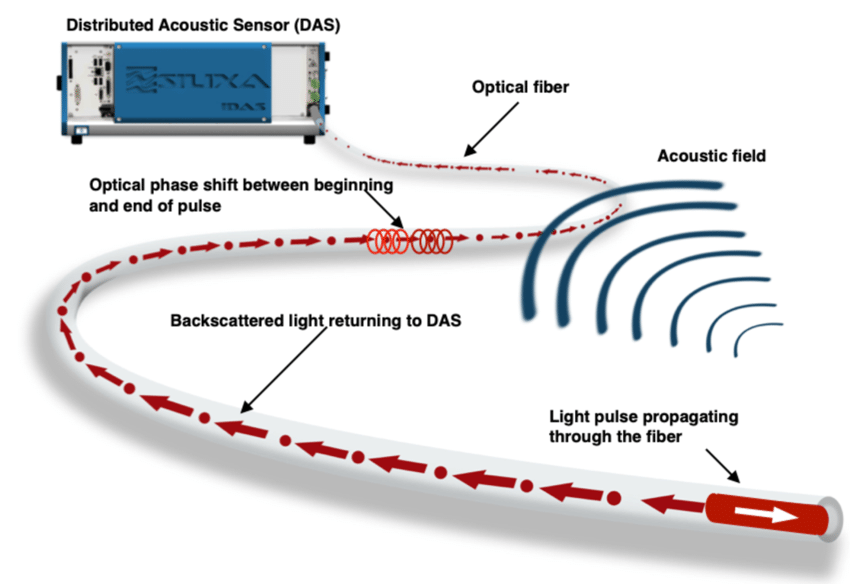
\includegraphics[width=0.7\linewidth]{figures/das.png}
    \caption{Showcase of how \acrshort{das} signals are recorded}
    \label{fig:das-fig}
\end{figure}



\section{Motivation}

Digital signal processing has over the last 100 years gone from almost non-existent to utmost critical importance. By processing signal data, one can get access to all kinds of information, music, movement and locations. There are tons of different devices for recording signals from the environments. From more well known ones such as microphones and sensors, to less commercial technologies.

The world of digital signal processing is nothing new to academia, and computer science in general. Some of the most magnificent and trailblazing algorithms, like the \acrfull{dft} algorithm revolve around solving problems revolving around these data. With more and more sensors being used around us, as well as the increasing amount of data stored, the larger the need for processing and interpreting this data has become. 
\acrfull{das} is a rather new technology that allows for real-time analysis over fiber-optical cables, and gives us highly sensitive senor data to work with. \acrshort{das} has gained more recognition. \\

It is hard to underestimate the impact \acrshort{ai} has had upon the general population this last couple of years. Ever since OpenAI released ChatGPT the 30th of november 2022 \cite{chatgpt} the amount of \acrshort{ai} technology and applications has exploded, not only large language models (\acrshort{llm}), but other domains have garnered attention as well. \acrshort{llm}s made \acrfull{rnn} more popular than they had been for a while. These models are good at remembering information, making current desicions based on previous ones. \\ 

\acrshort{das} technology in itself has now started garnering attention for research, and several papers have previously studied  how one can process this data. \acrshort{ai} and \acrshort{ml} models have been constructed for looking at time series data, and analyzing sensor data, although several of theses have studied .  Only recently has \acrshort{ai}

Anomaly detection on \acrshort{das} data 

Unsupervised learning has in later years returned after the explosion of generatiive models. They are well suited for detecting novel anomalies \cite{wei2022lstmautoencoder} \cite{srivastava2016unsupervised} and do not require labeling of data, something that can rather dificult on DAS data. Both GANs, AE, and LSTM VAE have been proven to have good metrics for determining anomalies. 


Python has for a long been the \textit{de-facto standard} language both for \acrshort{ai}, \acrshort{ml} and data analysis. All kinds of heavy pre-processing of data before training the data is being written in C or C++ or other more performant languages.    




Previous work on this data (see \cite{projthesis}) revolved around processing \acrshort{hdf5} files as fast and efficient as possible, trying to parallellize already existent code, and take advantage of newer technologies, such as Julia.

\subsection{NTNU SFI Center for Geophysical Forecasting}



We hereby present \texttt{JudasNET}, a LSTM VAE network written in Julia for anomaly detection on \acrshort{das} data. Additionally, we present \texttt{Judas - (Julia \& DAS)}, a Julia package containing functions for parsing HDF5 files, signal processing methods specifically for DAS sensor data, as well as functions for training, inference and utilities for AI models related to DAS data. As a sideeffect, we also show how Julia can be used effectively within multiple different fields to enable , and be easily tuned to their needs,
\section{Goals}

Given the vast scope and multiple facets of our project, it is important to clarify the specific objectives we aim to achieve with this thesis. Our goals are as follows:

\begin{enumerate}
    \item \textbf{Evaluating Julia for Big Data Science Applications}: Determine whether Julia is a suitable programming language for big data, data science and \acrshort{ai} applications
    \item \textbf{Assessing Autoencoders for Anomaly Detection in \acrshort{das} Data}: Evaluate the effectiveness of autoencoders in detecting anomalies within \acrshort{das} data, both in online and offline data.
    \item \textbf{Open Source Contributions for \acrshort{das}}: Contribute to the open-source community, particularly with tools and resources that are beneficial to members of \acrshort{cgf}.
\end{enumerate}


\subsection{Research Questions}

In addition to our goals, the following are a set of research questions we want answers to by the end of the thesis:

\begin{enumerate}
    \item \textbf{Scalability and Parallelization in \acrshort{das} Data Processing}: Can we develop a program that is both scalable and parallelizable for processing and training large \acrshort{hdf5} files?
    \item \textbf{Float16 Processing on \acrshort{das} data}: Can we reduce the precision of \acrshort{das} data to enable faster model training and inference without sacrificing performance?
\end{enumerate}

\section{Research Questions and Contributions}
\label{intro:contribs}

The following list provides the research questions of this thesis: 

\begin{enumerate}
    \item How do the spatial characteristics of \acrshort{das} data impact the performance of autoencoders for anomaly detection?
    \item What autoencoder architectures are most effective for anomaly detection in \acrshort{das} data when computational resources can be limited?
    \item What preprocessing techniques can optimize the efficiency-accuracy trade-off in anomaly detection of \acrshort{das} data?
\end{enumerate}

In this thesis, we study processing and autoencoder-based anomaly detection using \acrshort{das} data. Our work has led to several contributions, including:

\begin{itemize}
    \item \textbf{Autoencoder based anomaly detection}: We compare the effectiveness of different autoencoders for anomaly detection on dense \acrshort{das} data. In particular, we explore the spatial characteristics of in \acrshort{das} data.
    \item \textbf{Julia for data science and \acrshort{ai}}: We evaluate Julia as a programming language for developing high-performance applications and \acrshort{ai} programming.
    \item \textbf{Software}: The following software has been produced as a part of this thesis:
    \begin{itemize}
        \item \textbf{Judas}: A software package developed in Julia for processing \acrshort{das} data. Initially introduced in our project thesis \cite{projthesis}, Judas is now fully operational but only available for members of \acrshort{cgf}. 
        \item \textbf{TinyDAS}: An open-source program written in Python, specifically designed for training and evaluation of autoencoder models, as well as performing anomaly detection on \acrshort{das} data \footnote{\url{github.com/Jafagervik/TinyDAS}}. This program contains code and hyperparameters for 4 different autoencoders.  We establish how Tinygrad \cite{tinygrad} as a software package can be used to create hardware agnostic \acrshort{ai} programs that are scalable across multiple accelerators without changing source code. 
        \item \textbf{JudasNET}: An open-source repository with examples of autoencoders written in Julia \footnote{\url{github.com/Jafagervik/JudasNET}}.
    \end{itemize}
\end{itemize}

Overall, we seek to improve \acrshort{das} data processing and compare the effectiveness of smaller autoencoder models for anomaly detection on this data. In particular, we hope that members of \acrshort{cgf} can use and improve these tools to further \acrshort{das} research.
\section{Thesis outline}

The following list is an outline over the rest of the thesis, and what will be presented for each chapter. \\

%\textbf{Chapter 1: Introduction} - We present the problems, what we want to find out and our motivation for this project. \\

\textbf{Chapter 2: Background and Related Work} - We cover theory regarding \acrshort{das} processing techniques, both relevant \acrshort{dl} architectures and their applications to our problems, as well as some introduction to applicable signal processing techniques. Finally, we discuss relevant literature and work.  \\

\textbf{Chapter 3: Method} - We cover all our practical work and implementation decisions of both programs, including program design, data processing methods, and network architectures. \\

\textbf{Chapter 4: Experiments} - We present our experiments, covering datasets, the experiments scopes, as well as evaluation metrics and experiment setup. \\

\textbf{Chapter 5: Experimental Results} - We present our results from the experiments conducted in the Chapter 4. \\

\textbf{Chapter 6: Discussion} - We discuss the overall findings and results of our experiments. Furthermore, we discuss the current capabilities of our programs, including limitations, and answer our overarching goals. Finally, we discuss both enhancing qualities of the Julia programming language, as well as current limitations within \acrshort{ai} programming. \\

\textbf{Chapter 7: Conclusion and Further Work} - This final chapter concludes our thesis. We conclude our findings and discuss further work. \\

\textbf{Overlap with Project thesis}

Parts of this thesis are based on my submitted project assignment in TDT4501 titled "Parallel DAS Processing: Julia is all you need". Section \ref{met:Judas} is a continuation of previous work conducted in the project thesis \cite{projthesis}. We provide a clear distinction of what has been done before and what's new in regard to Judas (fka. Emerald). Section \ref{met:Julia} is a summarization of an introduction to Julia, previously covered in Section 2.1 of the project thesis. Section "Reflections on Julia" in Chapter 7 covers some of the previous talking points in the project thesis, but the subsection about Julia for \acrshort{ai} programming is new.
